\documentclass[10pt,a4paper]{article}
\usepackage[utf8]{inputenc}
%\usepackage[engl]{babel}
\usepackage[T1]{fontenc}
\usepackage{amsmath}
\usepackage{amsfonts}
\usepackage{amssymb}
\usepackage{graphicx}
\usepackage{bm}
\usepackage[rmargin=1.5cm, lmargin=1.5cm, bmargin=2cm, tmargin=2cm]{geometry}
\usepackage{enumitem}
\setitemize{noitemsep,topsep=0pt,parsep=0pt,partopsep=0pt}


\author{Lars Schiller}
\title{Algorithm for predicting the pose of a gecko-inspired soft robot for a given reference input}


\usepackage{multicol}

\newcommand{\mbeq}{\overset{!}{=}}

\begin{document}


\maketitle

Due to the fact that the behaviour of soft materials is difficult to predict with conventional methods, an algorithm based on a geometric optimization problem is presented.
The algorithm can be used to predict the actual pose of the robot for a given reference input.
Figure~\ref{fig:example} is taken as an example. The initial position is shown in black. 
The individual limbs of the robot have a certain bending angle and all feet are fixed.
Now the torso of the robot should be actuated. 
If only the bending angle of the torso is changed, the grey dashed pose is obtained. 
Obviously, the two rear feet are no longer in the same position. 
Since these feet are fixed, the robot will behave differently in reality. 
In fact, it's much more likely to take up the grey pose. 
Although the bending angles of all limbs have changed, the condition that all feet remain motionless has been fulfilled.

\begin{figure}[h]
\centering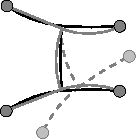
\includegraphics[scale=1]{../Pics/intro/intro.pdf}
\caption{Example Usage}
\label{fig:example}
\end{figure}


\section{Predicting the pose for a given reference input}
In order to let the robot take a pose
%, i.\,e., a position and orientation, 
the user has nine degrees of freedom at his disposal: 
the correspondending pressures for the five bending angles $\alpha_i$ of the limbs $i=1,\dots,5$ and the state of the fixation actuators $f_j \in \{0,1\}$ of the feet $j=1,\dots,4$.
For the unloaded state, a calibration function can be formulated for each limb, which maps the input pressure on the bending angle (under load, this function no longer needs to be valid).
But the input pressure can be seen as an reference for the bending angle.
Accordingly, a reference input $\bm{r}$ can be described by

\begin{equation}
\bm{\alpha}_{\textnormal{ref}} = \left[~ \alpha_{\textnormal{ref},1}~\alpha_{\textnormal{ref},2}~\alpha_{\textnormal{ref},3}~\alpha_{\textnormal{ref},4}~\alpha_{\textnormal{ref},5}~\right]^\top
\end{equation}

\begin{equation}
\bm{f} = \left[~f_1~f_2~f_3~f_4~\right]^\top
\end{equation}


\begin{equation}
\bm{r} = \left[~\bm{\alpha_{\textnormal{ref}}}^\top~\bm{f}^\top~\right]^\top.
\end{equation}

%
%\begin{equation}
%\alpha_{\textnormal{clb},i} = \textnormal{map}_i(p_i)
%\end{equation}

However, this information is not sufficient to describe the robot's actual pose.
%The exact position and orientation of at least one foot must be known.
Experiments have shown that the bending angle of a limb can vary significantly  at the same pressure level due to the softness of the used material. 
The length of a limb can also differ.
In order to describe the pose of the robot, the actual bending angles $\bm{\alpha}$: 
\begin{equation}
\bm{\alpha} = \left[ \alpha_1~\alpha_2~\alpha_3~\alpha_4~\alpha_5 \right]^\top,
\end{equation}
the actual lengths of the individual limbs $\bm{\ell$}: 
\begin{equation}
\bm{\ell} = \left[ \ell_1~\ell_2~\ell_3~\ell_4~\ell_5 \right]^\top,
\end{equation}
and the orientation of the robot's center point $\varepsilon$ must be known (see Fig.~\ref{fig:model}).
These quantities are defined as the variable to be optimized:
\begin{equation}
\bm{x} = \left[~\bm{\alpha}^\top~\bm{\ell}^\top~\varepsilon~\right]^\top.
\end{equation}

Furthermore, the position of (at least) one fixed foot ($f_j \mbeq 1$) must be known.
Then, the pose of the robot $\bm{\rho}$ can be determined under the assumption of a constant curvature by drawing arcs with the corresponding lengths and angles.
A pose can therefore be described in generally as a function of $\bm{x}$ and the position 
$\bm{P}=[\bm{p}_1~\bm{p}_2~\bm{p}_3~\bm{p}_4]^\top \in \mathbb{R}^{4 \times 2}$ and state $\bm{f}$ of all feet:
\begin{equation}
\bm{\rho} = \left[\bm{x},~\bm{P},~\bm{f} \right].
\end{equation}

\begin{figure}
\centering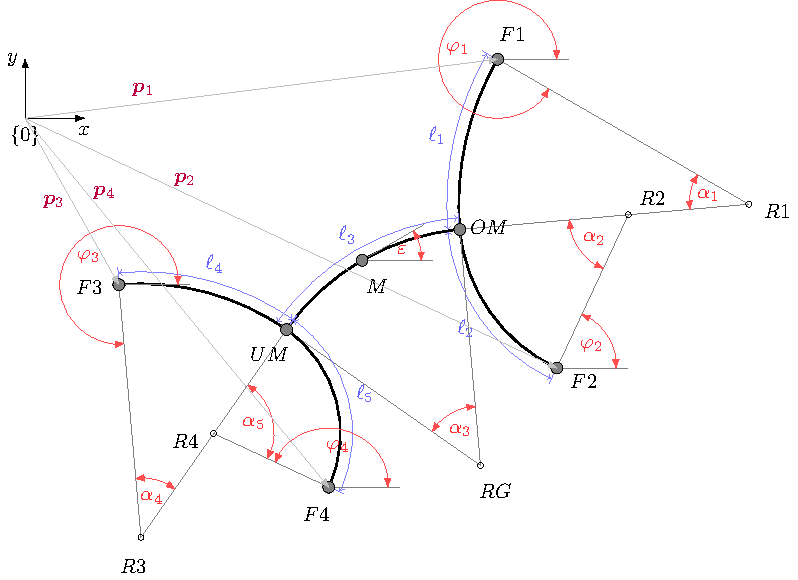
\includegraphics[scale=1]{../Pics/model/model.pdf}
\caption{Nomencalture}
\label{fig:model}
\end{figure}

For a given feasible initial pose, the next pose must be determined so that all fixed feet do not move.
This can be achieved within a certain margin by deviating the bending angle from the reference angle and deviating the actual length from the nominal length.
To describe this mathematically, a new index $k$ is introduced, which assigns the quantities to a specific time step.
The new positions of the fixed feet $\bm{P}_{k}$ are assumed to be the positions from the previous pose $\bm{P}_{k-1}$.
This can be used to define the constraint for the next pose.
All newly fixed feet must have the same position as in the previous step:
\begin{equation}
\big|\big|\textnormal{diag}(\bm{f}_k)(\bm{P}_{k} - \bm{P}_{k-1})\big|\big|_2 \mbeq 0,
\label{eq:constraint}
\end{equation}


%\begin{equation}
%\bm{p}_k \left(\bm{x},~\bm{p}_{k-1},~\bm{f}_k \right).
%\end{equation}

%Please note that if this condition is met, at least one foot per time step always remains motionless.
%Thus, at least one foot position of the new pose is determined from the beginning and thus dependent on the previous pose.
%As a result, all poses of a gait are dependent on the initial position.
%\begin{equation}
%\bm{\rho}_t = \textnormal{fun}\left(\bm{x}_t,~\bm{r}_{j,0} \right).
%\end{equation}

It has already been mentioned that the bending angles $\bm{\alpha}$ and the lengths of the limbs $\bm{\ell}$ are quite variable. 
By defining 
\begin{equation}
\bm{\ell}_n = \left[ \ell_{n,1}~\ell_{n,2}~\ell_{n,3}~\ell_{n,4}~\ell_{n,5} \right]^\top
\end{equation}
as the vector containing the nominal length of each limb, it is possible to quantify the length deviation.
The orientation angles of the fixation actuators $\bm{\varphi}$ also have a certain margin.
The value of the orientation angles can be calculated as a function of $\bm{\alpha}$ and $\varepsilon$ (well, basically as a function of $\bm{x}$):
\begin{equation}
\bm{\varphi}(\bm{\alpha}, \varepsilon) = \eqref{eq:phi_calc},
\end{equation}
where the exact formula is given in the appendix~\ref{eq:phi_calc}.
Now a objective function can be formulated which quantifies the deviations of length, angle and orientation:
%\begin{equation}
%obj(\bm{x}) = w_{len}\sqrt{\sum_i \left( \ell_{n,i} - \ell_i \right)^2} 
%+ w_{ang} \sqrt{\sum_i \left( \varphi_i - \alpha_i \right)^2}
%+ w_{ori} \sqrt{\sum_i \textnormal{if}~f_i:~\left( c_{i,j-1} - c_{i, j} \right)^2}
%\label{eq:objective_function}
%\end{equation}

\begin{equation}
obj(\bm{x}_{k}) = %, \bm{\varphi}_{k-1}) = 
  w_{\textnormal{len}}\big| \bm{\ell}_{k} - \bm{\ell}_n \big|_2
+ w_{\textnormal{ang}}\big| \bm{\alpha}_{k} - \bm{\alpha}_{\textnormal{ref},k} \big|_2
+ w_{\textnormal{ori}} \big| \textnormal{diag}(\bm{f}_k) ( \bm{\varphi}_{k} - \bm{\varphi}_{k-1}) \big|_2 .
\label{eq:objective_function}
\end{equation}
The weighting factors can be interpreted physically.
To do so, the weighting factor $w_{\textnormal{len}}$ describes the elasticity of the limbs and $w_{\textnormal{ang}}$ the bending stiffness of the limbs.
The term weighted by $w_{\textnormal{ori}}$ describes the difference between the orientation of the newly fixed feet compared to the orientation in the previous time step.
This can be seen as a dimension for the torsional stiffness of the fixation actuators.
The new pose can now be determined by solving the non-linear optimization problem:

\begin{equation}
\begin{split}
&\min_{\bm{x}_k \in \mathcal{X}} ~ obj(\bm{x}_k) \\
&subjected~to~~~
\big|\big|\textnormal{diag}(\bm{f}_k)(\bm{P}_{k} - \bm{P}_{k-1})\big|\big|_2 = 0.
\end{split}
\end{equation}
Here  $\mathcal{X}$ describes the set of allowed values.
Each quantity inside $\bm{x}$ has bounds, which are given in the following table:

\begin{center}
\begin{tabular}{c|c|c|c}
var & $\bm{\alpha}$ & $\bm{\ell}$ & $\varepsilon$ \\ 
\hline
bounds & $\left[ \bm{\alpha_{\textnormal{ref}}}-b_{\textnormal{ang}},~\bm{\alpha_{\textnormal{ref}}}+b_{\textnormal{ang}} \right]$ &
$\left[ (1-b_\textnormal{len})\bm{\ell}_n,~(1+b_\textnormal{len})\bm{\ell}_n \right]$ &
$\left[ 0^\circ,~ 360^\circ \right]$
\end{tabular}
\end{center}
These bounds can be tuned with the scalars $b_{\textnormal{ang}}$ and $b_{\textnormal{len}}$.
For solving the problem, for example the \texttt{SLSQP}-Algorithm provided by the python package \texttt{scipy.optimize} can be used.
Note that the evaluation of the objective function~\eqref{eq:objective_function} is quite cheap. 
The expensive part is the evaluation of the constraint function~\eqref{eq:constraint}, since the calculation of all feet positions for a given $\bm{x}$ is opulent and outlined in the appendix~\eqref{eq:F1_start}.

In summary, it is possible to set up a function that can predict the next pose of the robot, depending on the reference input and the previous pose:
\begin{equation}
\bm{\rho}_k = \textnormal{fun}\left( \bm{r}, \bm{\rho}_{k-1} \right)
\end{equation}
This function can be tuned by the parameters given in the following table:
\begin{center}
\begin{tabular}{l|l}
param & description \\
\hline
$b_{\textnormal{ang}}$ & allowed absolute deviation of the bending angle to the reference angle \\
$b_{\textnormal{len}}$ & allowed percentage deviation of the length to the nominal length \\
$w_{\textnormal{len}}$ & costs of the length deviation \\
$w_{\textnormal{ang}}$ & costs of the bending angle deviation\\
$w_{\textnormal{ori}}$ & costs of the orientation angle deviation\\
\end{tabular}
\end{center}



\section{Finding optimal gait patterns}

%Der vorgesttele Algorithmus kann nun dazu verwendet werden neue Laufmuster zu finden.
%Da er die Möglichkeit bietet vorherzusagen, welche Pose der Roboter bei gegebenem Referenz Input einnehmen wird, ist er durch rekursive Anwendung in der Lage alle zugehörigen Posen des Roboters zu einer Sequenz von Referenz Inputs zu prädiktieren.
%
%Ein Laufmuster besteht aus einer ebensolchen Sequenz aus Posen, die in Dauerschleife eingenommen werden.
%Um nun eine optimale Abfolge von Referenz Inputs zu finden, muss erst einmal definiert werden, was optimal ist.
%Dies kommt ganz darauf an, welche Art von Laufmuster gesucht wird. 
%im Folgenden werden zwei Beispiele vorgestellt.

The presented algorithm can now be used to find new gait patterns.
Since it provides the ability to predict the robot's pose for a given reference input, it is able to predict all associated poses to a sequence of reference inputs by recursive application.

A gait pattern consists of a sequence of poses taken in a continuous loop.
To find an optimal sequence of reference inputs, it is first necessary to define what is optimal.
This depends entirely on the type of running pattern you are looking for. 
Two examples are presented below.

\subsection{Straight Gait}

Soll der Roboter geradeaus Laufen, so ist es optimal die Distanz von Startpunkt und Endpunkt möglichst zu maximieren.

\begin{equation}
\bm{x} = \begin{bmatrix}
\bm{r}_1^\top \\ \bm{r}_2^\top
\end{bmatrix}
=
\begin{bmatrix}
\alpha_{\textnormal{ref},1}& \alpha_{\textnormal{ref},2}&\alpha_{\textnormal{ref},3}&\alpha_{\textnormal{ref},4}&\alpha_{\textnormal{ref},5}&1&0&0&1 \\
\alpha_{\textnormal{ref},2}& \alpha_{\textnormal{ref},1}&-\alpha_{\textnormal{ref},3}&\alpha_{\textnormal{ref},5}&\alpha_{\textnormal{ref},4}&0&1&1&0 \\
\end{bmatrix}
\end{equation}


\subsection{Gait Pattern for a curve}


\appendix
\section{Appendix}

\begin{multicols}{2}

Coordinates for $F1$ fixed:

\begin{equation}
r_i = \frac{360 ~ \ell_i}{2 \pi ~ \alpha_i},~~ \textnormal{for}~ i \in [1,2,3,4,5]
\end{equation}

\begin{equation}
\bm{\varphi} = \begin{bmatrix}
\varepsilon - \alpha_1 - \frac{1}{2}\alpha_3 \\
\varphi_1 + \alpha_1 + \alpha_2 \\
180^\circ + \alpha_3 - \alpha_2 + \alpha_4 + \varphi_2 \\
180^\circ + \alpha_3 - \alpha_1 + \alpha_5 + \varphi_1 \\
\end{bmatrix}
\label{eq:phi_calc}
\end{equation}


\begin{equation}
\label{eq:F1_start}
R1 =  \begin{bmatrix} 
F1_x +\cos(c_1)~r_1 \\ 
F1_y + \sin(c_1)~r_1\end{bmatrix}
\end{equation}

\begin{equation}
OM =  \begin{bmatrix} 
R1_x - \sin(90-c_1-\alpha_1)~r_1 \\ 
R1_y - \cos(90-c_1-\alpha_1)~r_1 \end{bmatrix}
\end{equation}

\begin{equation}
RG =  \begin{bmatrix} 
OM_x + \cos(90-c_1-\alpha_1)~r_\gamma \\ 
OM_y - \sin(90-c_1-\alpha_1)~r_\gamma \end{bmatrix}
\end{equation}

\begin{equation}
UM =  \begin{bmatrix} 
RG_x - \cos(\gamma - 90 + c_1 + \alpha_1)~r_\gamma \\ 
RG_y - \sin(\gamma - 90 + c_1 + \alpha_1)~r_\gamma \end{bmatrix}
\end{equation}

\begin{equation}
R4 =  \begin{bmatrix} 
UM_x + \sin(\gamma - 90 + c_1 + \alpha_1)~r_4 \\
UM_y - \cos(\gamma - 90 + c_1 + \alpha_1)~r_4 \end{bmatrix}
\end{equation}

\begin{equation}
F4 =  \begin{bmatrix} 
R4_x + \sin(-c_4-90)~r_4 \\
R4_y + \cos(-c_4-90)~r_4 \end{bmatrix}
\end{equation}

\begin{equation}
R3 =  \begin{bmatrix} 
UM_x + \sin(\gamma - 90 + c_1 + \alpha_1)~r_3 \\
UM_y - \cos(\gamma - 90 + c_1 + \alpha_1)~r_3 \end{bmatrix}
\end{equation}

\begin{equation}
F3 =  \begin{bmatrix} 
R3_x - \cos(-c_3)~r_3 \\
R3_y + \sin(-c_3)~r_3 \end{bmatrix}
\end{equation}


\begin{equation}
R2 =  \begin{bmatrix} 
OM_x + \cos(c_1 + \alpha_1)~r_2 \\
OM_y + \sin(c_1 + \alpha_1)~r_2 \end{bmatrix}
\end{equation}

\begin{equation}
F2 =  \begin{bmatrix} 
R2_x + \sin(c_2 - 90)~r_2 \\
R2_y - \cos(c_2 - 90)~r_2 \end{bmatrix}
\label{eq:F1_end}
\end{equation}



Coordinates for $F2$ fixed:


\begin{equation}
R2 = \begin{bmatrix}
F2_x - \sin(c_2 - 90)~r_2 \\
F2_y + \cos(c_2 - 90)~r_2
\end{bmatrix}
\end{equation}

\begin{equation}
OM = \begin{bmatrix}
R2_x - \sin(90- c_2 + \beta_1)~r_2 \\
R2_y - \cos(90- c_2 + \beta_1)~r_2
\end{bmatrix}
\end{equation}

\begin{equation}
RG = \begin{bmatrix}
OM_x + \cos(90- c_2 + \beta_1)~r_\gamma \\
OM_y - \sin(90- c_2 + \beta_1)~r_\gamma
\end{bmatrix}
\end{equation}

\begin{equation}
UM = \begin{bmatrix}
RG_x - \cos(\gamma - 90 + c_2 - \beta_1)~r_\gamma \\
RG_y - \sin(\gamma - 90 + c_2 - \beta_1)~r_\gamma
\end{bmatrix}
\end{equation}

\begin{equation}
R4 = \begin{bmatrix}
UM_x + \sin(\gamma - 90 + c_2 - \beta_1)~r_4 \\
UM_y - \cos(\gamma - 90 + c_2 - \beta_1)~r_4
\end{bmatrix}
\end{equation}

\begin{equation}
F4 = \begin{bmatrix}
R4_x + \sin(-c_4 -90)~r_4 \\
R4_y + \cos(-c_4 -90)~r_4
\end{bmatrix}
\end{equation}

\begin{equation}
R3 = \begin{bmatrix}
UM_x + \sin(\gamma - 90 + c_2 - \beta_1)~r_3 \\
UM_y - \cos(\gamma - 90 + c_2 - \beta_1)~r_3
\end{bmatrix}
\end{equation}

\begin{equation}
F3 = \begin{bmatrix}
R3_x - \cos(-c_3)~r_3 \\
R3_y + \sin(-c_3)~r_3
\end{bmatrix}
\end{equation}


\begin{equation}
R1 = \begin{bmatrix}
OM_x + \sin(90-c_2+\beta_1)~r_1 \\
OM_y + \cos(90-c_2+\beta_1)~r_1
\end{bmatrix}
\end{equation}


\begin{equation}
F1 = \begin{bmatrix}
R1_x - \sin(90-c_1)~r_1 \\
R1_y - \cos(90-c_1)~r_1
\end{bmatrix}
\label{eq:F2_end}
\end{equation}

\end{multicols}




\end{document}